\section{Ejercicio 3}
\subsection*{Instrucción}
Cuando los clientes de la empresa de alquiler de coches alquilan un coche, el sistema que estamos construyendo
tiene que proporcionarles el precio del alquiler. Este precio lo calcula la operación \texttt{getPrice() : Integer} de la siguiente
forma: El precio base será el precio del modelo del vehículo por día.
\begin{center}
    \texttt{ (pricePerDay) * [endDate - startDate]}
\end{center}
Además, la empresa de alquiler de coches puede añadir al cálculo de precios la posibilidad de hacer promociones
que implican descuentos de estos precios. Inicialmente, la empresa ofrecerá dos tipos de promociones: por cantidad
y por porcentaje.
\begin{itemize}
    \item \textbf{Promoción por cantidad:} permitirá decrementar el precio del alquiler en la cantidad indicada en
    la promoción.
    \item \textbf{Promoción por porcentaje:} decrementará el precio del alquiler en el porcentaje indicado en la
    promoción. Las promociones se asignan a los alquileres en el momento de su creación.
\end{itemize}
Evidentemente, es posible
que a algunos alquileres no se les aplique ninguna promoción. Las promociones que se asignan a los alquileres son
determinadas por una política de la empresa que no impacta al diseño de nuestra operación (impactará a la
operación que crea los alquileres).\par
\vspace{0.15cm}
Eso sí, la empresa quiere que mientras no se haga el pago del alquiler, si aparecen
nuevas promociones, se apliquen a los alquileres siempre y cuando sean más favorables (no nos tenemos que
preocupar tampoco de estos cambios, son gestionados por otras operaciones).


\subsection{Patrón de Diseño utilizado}
Para poder realizar este apartado optamos varias casuísticas de diferentes patrones de diseño validos. Por un lado optamos por el patron visitante,
dicho patron complicaría demasiado la implementación de la operación debido al gran numero de instancias presentes de dicho patron para un unico método,esto hace que 
el uso de este patron sea algo ineficiente. Tras ese planteamiento llegamos a la conclusion de utilizar el patron \textbf{Strategy} para poder implementar la operación correctamente.
Este patron se basa en la utilización de una interfaz que actúa como padre de todos los objetos que implementen una operación similar, en este caso tenemos dos tipos de promociones,
\textbf{Promoción por porcentaje} y \textbf{Promoción por cantidad} ambas mantienen una lógica similar por lo que el uso del patron \textbf{Strategy} es el adecuado.

\subsection{Efectos sobre el Diagrama de Diseño}

\begin{figure}[H]
    \centering
     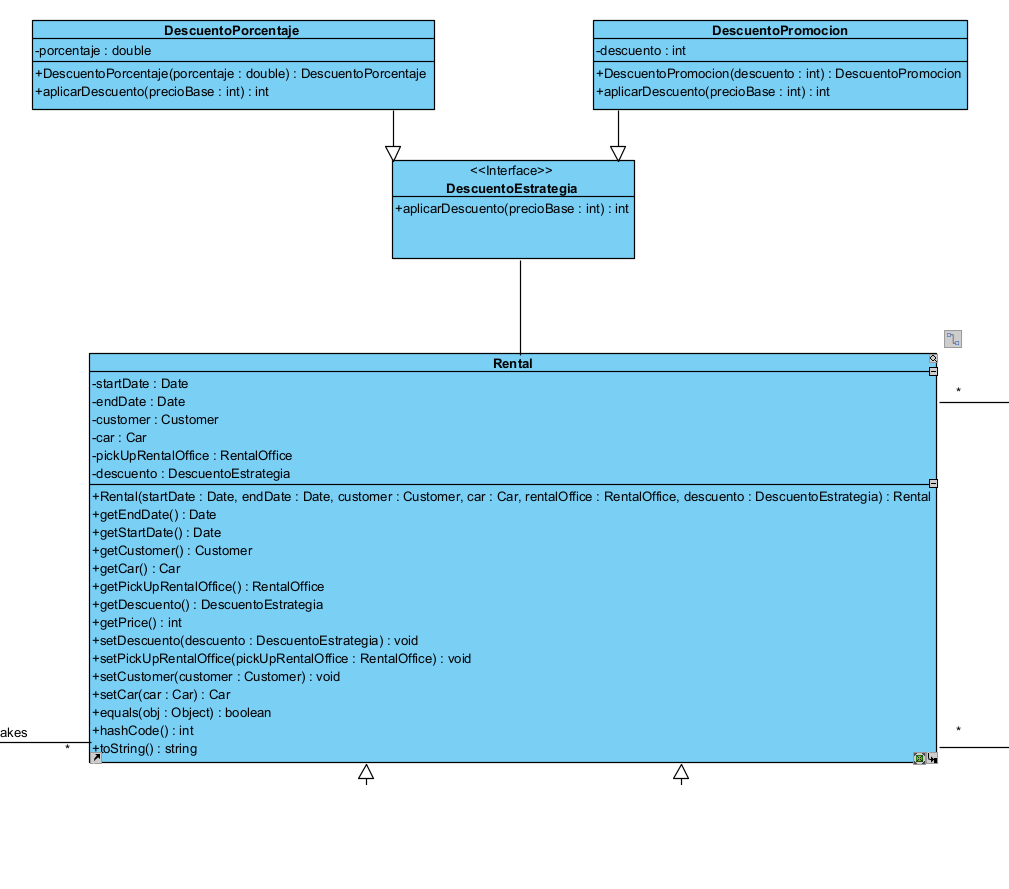
\includegraphics[width=1\linewidth]{assets/diagramas/UML_Apartado3.png}
     \caption{Diagrama de Diseño del apartado 3}
\end{figure}

Como podemos observar, el patron \textbf{Strategy} mantiene una interfaz padre de la cual heredan todas las instancias de objetos que vayan a realizar dicha operación.
Como bien hemos dicho antes nos basamos en un sistema con dos operaciones diferentes para obtener el precio final, por lo cual necesitaremos crear dos clases una para cada tipo de 
promoción. Estas heredaran de la clase \textbf{Strategy} para asi obligar al sistema a implementar dichas operaciones en cada una de las clases. Un requisito del sistema es que dichas
promociones se apliquen al instanciar un objeto \textbf{Rental}, es por eso que dichos tipos de promociones vendrán instanciados en el constructor de dicha clase pudiendo ser nulo en caso 
de que no se le aplique ningún tipo de promoción.\par
\newpage
\subsection{Implementación de \textit{getPrice() : Integer}}
\begin{lstlisting}[style = javaNormal, language=Java] 

    introducir codigo aqui

\end{lstlisting}\par
En la primera sección podemos encontrar las nuevas instancias que debemos generar para poder usar el patron \textbf{Strategy} dichas clases implementan el método de la interfaz
de manera similar pero cambiando ligeramente la forma en la que calculan los precios a dependiendo de sus propios parámetros privados (porcentaje o cantidad).\par
\vspace{0.15cm}
Para implementar el método getPrice hemos decidido generar a partir de los parámetro \textbf{startDate} y \textbf{endDate} el precio base que tendría el alquiler antes de aplicar 
cualquier tipo de promoción. Como bien hemos explicado antes en caso de que no exista promoción alguna se instanciará como nulo el atributo en el constructor. Es por eso que 
antes de calcular el nuevo precio comprobamos si el \textbf{Rental} contiene un tipo de promoción disponible, en caso contrario devolveremos el precio base inicial.

\newpage

\subsection{Ejemplo de ejecución}
\subsubsection*{Código del tester}
\begin{lstlisting}[style = javaNormal, language=Java] 
    // Crear modelos de coches
    Model modelA = new Model("Model A", 50);
    Model modelB = new Model("Model B", 70);

    // Crear oficinas de alquiler
    RentalOffice office1 = new RentalOffice("Office 1", 20);
    RentalOffice office2 = new RentalOffice("Office 2", 25);
    // Crear coches
    Car car1 = new Car("ABC-123", modelA, office1);
    Car car2 = new Car("XYZ-789", modelB, office2);

    // Crear clientes
    Customer customer1 = new Customer("12345678A", "Alice");

    // Alquiler con fechas solapadas
    Date startDate1 = new GregorianCalendar(2024, Calendar.JANUARY, 1).getTime();
    Date endDate1 = new GregorianCalendar(2024, Calendar.JANUARY, 10).getTime();
    Date startDate2 = new GregorianCalendar(2024, Calendar.JANUARY, 5).getTime(); // Solapado
    Date endDate2 = new GregorianCalendar(2024, Calendar.JANUARY, 15).getTime();
    DescuentoPorcentaje descPorcentaje = new DescuentoPorcentaje(50);
    DescuentoPromocion descPromocion = new DescuentoPromocion(100);
    Rental rental1 = new RentalOnSite("First rental", startDate1, endDate1, customer1, car1, office1,descPorcentaje);
    Rental rental2 = new RentalOnSite("Overlapping rental", startDate2, endDate2, customer1, car1, office1,descPromocion);

    // Mete alquileres al cliente
    customer1.addRental(rental1);
    customer1.addRental(rental2); // Esto viola la restriccion de solapamiento

    // Alquiler con fecha de inicio posterior a la fecha de finalizacion
    Date invalidStartDate = new GregorianCalendar(2024, Calendar.FEBRUARY, 10).getTime();
    Date invalidEndDate = new GregorianCalendar(2024, Calendar.FEBRUARY, 5).getTime(); // Invalido

    Rental invalidRental = new WebRental(11, invalidStartDate, invalidEndDate, customer1, car2, office2,null);

    // Alquiler web con hora de entrega despues de las 13:00
    Rental lateDeliveryRental = new WebRental(14, startDate1, endDate1, customer1, car2, office1,null); // Invalido

    // Mete mas alquileres
    customer1.addRental(invalidRental);
    customer1.addRental(lateDeliveryRental);

    // Imprimir resultados
    System.out.println("Customer Rentals:");
    System.out.println(customer1);

    System.out.println("\nOffice Rentals:");
    System.out.println(office1.toString());
    System.out.println(office2.toString());
    //Comprobar que los precios han cambiado en base a la promocion dada en el sistema
    System.out.println("----------------------------------------------------------------");
    System.out.println("Precio tras aplicar un descuento del " + rental1.getDescuento().toString() + " del tipo " + rental1.getDescuento().getClass().getName() + ": " + rental1.getPrice() + "\n");
    System.out.println("Precio tras aplicar un descuento del " + rental2.getDescuento().toString() + " del tipo " + rental2.getDescuento().getClass().getName() + ": " + rental2.getPrice() + "\n");
\end{lstlisting}


\subsubsection*{Output}

\begin{lstlisting}[style = javaNormal, language=Java] 
    Precio tras aplicar un descuento del [50.0] del tipo DescuentoPorcentaje: 225

    Precio tras aplicar un descuento del [100] del tipo DescuentoPromocion: 400
\end{lstlisting}

\vspace{1cm}

\newpage

Los \texttt{toString()} usados para mostrar el Output fueron:

\begin{lstlisting}[style = javaEspecifico, language=Java] 
    // en DescuentoPromocion
    @Override
    public String toString() {
        return "[" + descuento + "]";
    }

    // en DescuentoPorcentaje
    @Override
    public String toString() {
        return "[" + porcentaje + "]";
    }
\end{lstlisting}
